\documentclass[../main.tex]{subfiles}

\begin{document}
%%%%%%%%%%%%%%%%%%%%%%%%%%%%%%%%%%%%%%%%%%%%%%%%%%%%%%%
%   New Chapter                                       %
%%%%%%%%%%%%%%%%%%%%%%%%%%%%%%%%%%%%%%%%%%%%%%%%%%%%%%%

\chapter{Generative Models}
In this chapter, we will talk about another interesting thing that is happening in machine learning, particularly in deep neural models, the generative models. Our discussion contains three parts: Variational Autoencoders (VAEs),  Generative Adversarial Networks (GANs), and Autoregressive Models. The first two methods are a little bit involved with a bunch of mathematical derivations, while the last one is much more straightforward but still able to produce interesting results. 
\section{Motivation}
Let us start with some motivations. Figure \ref{fig_8_1} shows some recent results for face generating. It's based on 4 or 5 years works of the community on generative models. The looks quite amazing in a sense that even if us human are extremely suspicious about faces one can hardly tell that they are synthesized by computers. There's a lot of progress on voice synthesis as well, where people have be able to generate very human-like computer voice and can even imitate one's voice given only 30s voice sample.
\begin{figure}[h] 
	\centering 
	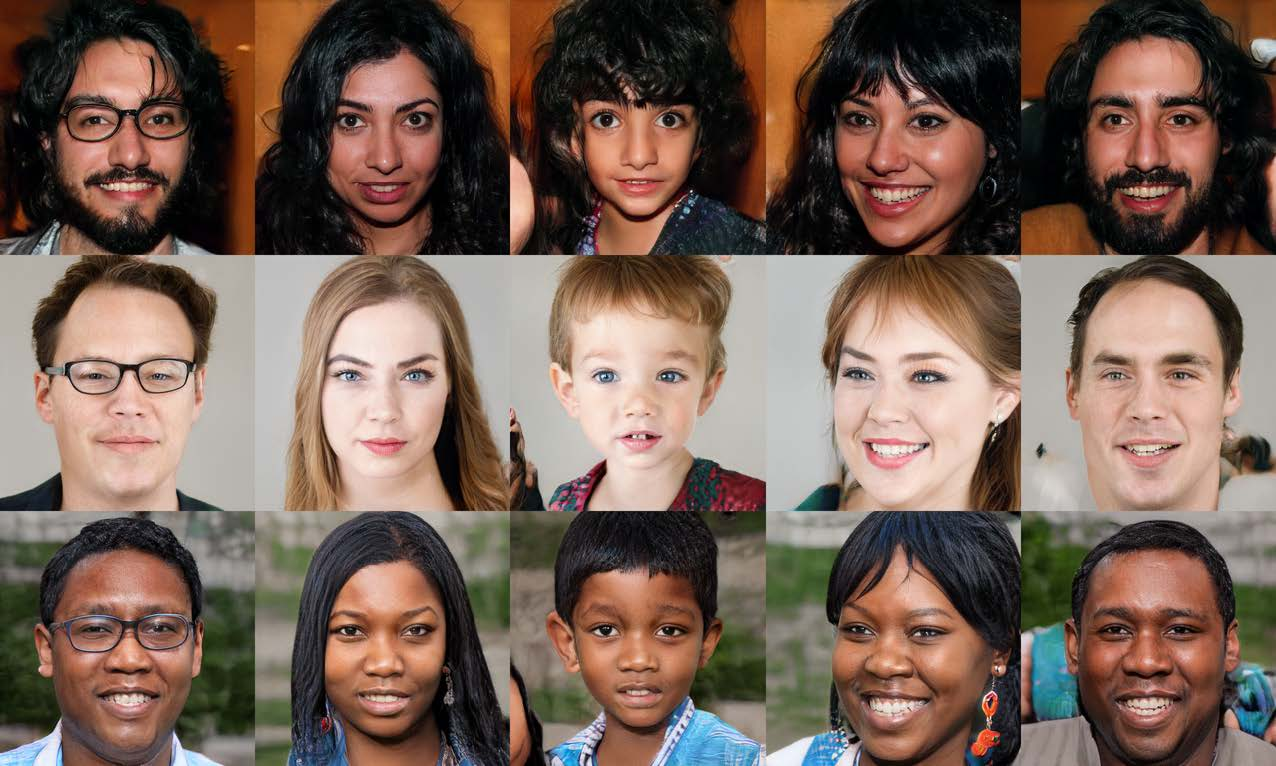
\includegraphics[width=8cm]{fig_8_1.jpg} 
	\caption{Faces generated by StyleGAN (NVIDIA), March 2020}\label{fig_8_1}
\end{figure}
\par Generally speaking, machine learning for synthesis (or generation) is more fascination than analysis (or recognition). If we have a generative model, rather than a discriminate model providing prediction for labels, we have much more details for what a computer has learned, and we are able to check where are the perceptible mistakes and improve our models. Recent developments in this area open up vastly new possibility for machine learning bringing breakthroughs in fields like animation, games, movies, art and mixed reality. Probably we are witnessing a revolution about how artificial worlds will be created, and how artificial things will be embedded into our real worlds. Though we are really only at the beginning, we will discuss several methods that we deal with in this fascinating area.
\section{Variational Autoencoders}
As the name suggests, VAEs is basically using the idea of Autoencoders (Chapter 1) that performs dimension reduction, take the data, compress it to some lower dimensional space, and then be able to reconstruct from that low dimensional thing. The key idea of VAEs, also GANs, is that if we want to sample or generate random things, we need to put some randomness into our mechanisms. 
\subsection{Deep Generative Models}
\par Since DNNs have the power to create complex distributions, we can start by sampling random vectors from a simple distribution, say a $m$-dimensional Gaussian: $\mathbb{R}^{m}\ni {\bf z}\sim \mathcal{N}(0,{\bf I})$ (it can be other distributions as well, it doesn't really matter). We then take this random vector, plug it into a network to output a sample, say an image. The idea is based on that DNNs can implement really complex transformations (recall that in image classification the learned mapping is from thousands of pixels to a single label). Here we go the other way: given a random vector, we use a deep network to transform it into something like a face, and if we sample the random vectors we sample in the face space. 
\par Formally, we want to transform random vectors though a (deterministic) deep network $F_{\theta}:\mathbb{R}^m\rightarrow\mathbb{R}^n$ parametrized by some $\theta$ with usually $n\gg m$. For example, with $n$, as the number of pixels in a image, say $40000$, $m$ might be only few hundreds. The distribution of ${\bf z}$ together with $F_{\theta}$ induce a (possibly complex) distribution over $\mathbb{R}^n$ with parameters $\theta$. This distribution is easy to sample: we can sample ${\bf x}$ by sampling ${\bf z}$ and setting ${\bf x}=F_{\theta}({\bf z})$. By the \emph{law of the unconscious statistician} we can compute the expectations over the induced distribution of any function $f({\bf x})$:
\begin{equation}\label{eq_8_lotus}
\mathbb{E}_{\bf x}[f({\bf x})]=\mathbb{E}_{\bf z}[f(F_{\theta}({\bf z}))].
\end{equation}
This proposition is known as the law of the unconscious statistician because students have been accused of using the identity without realizing that it must be treated as the result of a rigorously proved theorem, not merely a definition (comment from Wiki). A short proof for a invertable and differentiable $F_{\theta}({\bf z})$ with continuous random variables goes as follow (while the law holds for more general functions)
\begin{align*}
\mathbb{E}_{\bf x}[f({\bf x})]&=\int p_{\bf x}({\bf x})f({\bf x})d{\bf x}\\
&=\int \left|\frac{\partial F_{\theta}^{-1}({\bf x})}{\partial {\bf x}} \right|f({\bf x})p_{\bf z} (F_{\theta}^{-1}({\bf x})) d{\bf x}\ \text{(change of variables formula)}\\
&=\int p_{\bf z}({\bf z})f(F_{\theta}({\bf z}))d{\bf z}\ ({\bf z}=F_{\theta}^{-1}({\bf x}),\ d{\bf z}=\left|\frac{\partial F_{\theta}^{-1}({\bf x})}{\partial {\bf x}} \right|d{\bf x})\\
&=\mathbb{E}_{\bf z}[f(F_{\theta}({\bf z}))].
\end{align*}
According to (\ref{eq_8_lotus}), if we want to compute the expectation w.r.t. to the induced distribution over the high-dim space, we could get that expectation by sampling ${\bf z}$ from that simpler distribution, sending ${\bf z}$ through the mapping $F_{\theta}$, and averaging them. Why is this relevant? Because it says that to compute the expectations we don't need to know the density of ${\bf x}$ if we know the density of ${\bf z}$. Since in the discussions involving distributions, very often we need to compute expectations (usually via sample approximation) which can be obtained in this way, no matter what $f({\bf x})$ is.
\begin{remark}
	We know with the DNN, a distribution on a low-dimensional space induces a distribution over a higher-dimensional space. However, it's clear that it will not fill that space if $F_{\theta}$ is differentiable from ReLU and things we use. In general the network finds a manifold in that high-dim space, which actually makes sense since as mentioned, in many cases the data are believed to be highly structured in a sense that they lie in a manifold or are sparse in some basis (e.g. it is believed that natural images are sparse in wavelet basis as we will see in the following chapters). 
\end{remark}
\par Usually the way we think about statistical model for generating data is in terms of densities. Recall that we have a simple distribution over ${\bf z}$ with the corresponding generated data ${\bf x}$ (say a face) induced by a deterministic function $F_{\theta}$ implemented by a DNN: ${\bf x}=F_{\theta}({\bf z})$. Then if $F_{\theta}$ is invertable as well, we can compute the density of ${\bf x}$ in terms of the one of ${\bf z}$ by the \emph{change of variable formula}:
\begin{equation}\label{eq_8_chg_var}
{\bf x}=F_{\theta}({\bf z}),\quad \underbrace{p_{\bf x}({\bf x})}_{{\bf x}-\text{density}}=\left|\frac{\partial F_{\theta}^{-1}({\bf x})}{\partial {\bf x}}\right|\underbrace{p_{\bf z}(F_{\theta}^{-1}({\bf x}))}_{{\bf z}-{\rm density}}.
\end{equation}
Specifically, we would find the pre-image ${\bf z}$ that is mapped to ${\bf x}$ by $F_{\theta}$. Then we could compute the density of that pre-image ${\bf z}$, and then we adjust for the volume effect: how much distortion of the volume is locally happening, which is captured by the inverse Jacobian determinant. The density of ${\bf x}$ is useful since with it we can do things like maximum likelihood estimation given some real data by computing their likelihood function via (\ref{eq_8_chg_var}). However, in practice this will be problematic since it requires to 
\begin{itemize}
	\item find the network inversion
	\item compute the inverse Jacobian determinant
	\item compute gradients with respect to $\theta$ to learn,
\end{itemize}
some of which are often impossible (non-invertible) or intractable/impractical (dimensionality) avoiding the attempt to construct density directly. For simple $F$ this is okay, but for models we are interested in, i.e. deep models, this shows not much practical success.
\subsection{Evidence Lower Bound}
What can we do if the attempt to get density and evaluate the likelihood function doesn't work? One thing that does work is to apply the principle we have seen in the EM algorithm. In the context here, it refers to the variational lower bound or Evidence Lower BOund (ELBO). 
\par Specifically, instead of using a deterministic $F_{\theta}$, we relate ${\bf x}$ to ${\bf z}$ via a slightly more general way, a conditional distribution $p_{\theta}({\bf x}|{\bf z})$ parametrized by some $\theta$. This setting allows a little bit noise. Then together with the distribution of the latent variable $p({\bf z})$, we can define a complete data model that is given by
\begin{equation*}
p_{\theta}({\bf x},{\bf z})=p_{\theta}({\bf x}|{\bf z})p({\bf z}).
\end{equation*}
Integrating out ${\bf z}$ yields
\begin{equation*}
p_{\theta}({\bf x})=\int p_{\theta}({\bf x},{\bf z})d{\bf z} = \int p_{\theta}({\bf x}|{\bf z})p({\bf z})d{\bf z},
\end{equation*}
which is the marginal likelihood of ${\bf x}$. At this point, one might attempt to maximize the marginal likelihood directly, but we may not know how to perform the integration. Recall what we have seen in EM, to maximize the log marginal likelihood, we can maximize a lower bound of it instead. Again, we first introduce a variational distribution $q_{\phi}({\bf z};{\bf x})$ and rewrite the log-likelihood as
\begin{equation*}
\log p_{\theta}({\bf x})=\log \int q_{\phi}({\bf z};{\bf x}) \frac{p_{\theta}({\bf x}|{\bf z})p({\bf z})}{q_{\phi}({\bf z};{\bf x})}d{\bf z} = \log \mathbb{E}_{q_{\phi}} \left[\frac{p_{\theta}({\bf x}|{\bf z})p({\bf z})}{q_{\phi}({\bf z};{\bf x})}\right].
\end{equation*}
\begin{remark}
	In the CIL slides, the notation ($q_\phi({\bf z}|{\bf x})$ or $q_\phi({\bf z};{\bf x})$) is inconsistent. To avoid unnecessary confusions, we use the latter one for the whole chapter. However, as argued by one of the TAs on piazza, the notation $q_\phi({\bf z}|{\bf x})$ is improper. In the context of VAE, we assume two random variables: ${\bf x}$ (the data) and ${\bf z}$ (the latent variable). We also assume that the probability density function (pdf) they admit exist ($p({\bf x})$ and $p({\bf z})$). In VAE, we introduce a variational distribution $q_\phi({\bf z})$ to approximate the conditional distribution (or posterior) $p({\bf z}|{\bf x})$ which is called true precisely because it is induced by random variables ${\bf x}$ and ${\bf z}$. Note that even if $q_\phi({\bf z})$ might depend on ${\bf x}$ (since ${\bf x}$ is given, so we can write $q_\phi({\bf z};{\bf x})$) and $q_\phi({\bf z})$ is technically a distribution, it is not the conditional pdf $p({\bf z}|{\bf x})$ (unless they are the same almost everywhere) and it makes no sense to write it in a conditional form $q_\phi({\bf z}|{\bf x})$. In general
	\begin{equation*}
		p({\bf z}) = \int q_\phi({\bf z};{\bf x})p({\bf x})d{\bf x}
	\end{equation*}
	will not hold.
	%One can interpret it as the conditional distribution given ${\bf x}$ (as our VAE model is trying to model this), but as a variational distribution, it only has to be a distribution over ${\bf z}$ (that's why in PRML it just wrote $q_\phi({\bf z})$ instead). The notation of $q_\phi({\bf z};{\bf x})$ is just to emphasize it is a distribution over ${\bf z}$ with possible dependencies on ${\bf x}$.
\end{remark}
Use the concavity and apply the Jensen's inequality yields
\begin{align*}
\log p_{\theta}({\bf x})\geq {\rm ELBO}(\phi, \theta)&=\mathbb{E}_{q_{\phi}}\left[\log p_{\theta}({\bf x}|{\bf z}) + \log \frac{p({\bf z})}{q_{\phi}({\bf z};{\bf x})} \right]\\
&=\underbrace{\mathbb{E}_{q_{\phi}}\left[\log p_{\theta}({\bf x}|{\bf z})\right]}_{\rm predictiveness} - \underbrace{{\rm KL}(q_{\phi}({\bf z};{\bf x})||p({\bf z}))}_{\rm regularization},
\end{align*}
where ${\rm KL}(q||p)$ is the Kullback-Leibler divergence, which is a measure of distance between distributions. The term $-{\rm KL}(q_{\phi}({\bf z};{\bf x})||p({\bf z}))$ encorages the posterior distribution to be close to the prior distribution on the latent variable ${\bf z}$, which acts as a regularizer. The first term $\mathbb{E}_{q_{\phi}}\left[\log p_{\theta}({\bf x}|{\bf z})\right]$ maximizes the likelihood of ${\bf x}$, which is related to the reconstruction quality. Just as in EM, we can alternatively
\begin{itemize}
	\item maximize w.r.t. $\theta$ (generative model, given $q_{\phi}$), M step in EM;
	\item maximize w.r.t. $\phi$ (inference model, given $p_\theta$), E step in EM. 
\end{itemize}
For a discussion for general EM and what do E and M step do please refer to section \ref{sec_4_EM_in_gen}. Usually in E step maximizing  w.r.t. $\phi$ means we need to compute the posterior of latent variable $p_{\theta^{\rm old}}({\bf z}|{\bf x})$ w.r.t. the old parameters, but for deep models it's too complicated. Instead, we try to compute some approximation via updates with specifically designed $q_{\phi}$.
\par Before the discussion of how we can maximize w.r.t. $\theta$ and $\phi$, let us see the VAE in a big picture that is a bit more abstract. A typical VAE can be represented in a diagram shown in Figure \ref{fig_8_2}. The right half is the generative path, where we sample ${\bf z}$ and pass it through a network to generate data ${\bf x}$ (note that this is done by sampling from the distribution $p_\theta({\bf x}|{\bf z})$ determined by the generative model). The left half is the inference path, where we do the opposite: conditioning on a data point ${\bf x}$, we want to find good Gaussian vectors ${\bf z}$ for that data ${\bf x}$, which is done in a probabilistic way (output a distribution $q_{\phi}({\bf z};{\bf x})$ rather than a deterministic value). The inference model encodes ${\bf x}$ (probabilistically) as a vector ${\bf z}$ in a much more lower dimensional space, while the generative model decodes ${\bf z}$ to produce data point ${\bf x}$. During the train, since we do thing in an unsupervised manner, we want the loop to produce or approximate in some sense the identity mapping.
\begin{figure}[h] 
	\centering 
	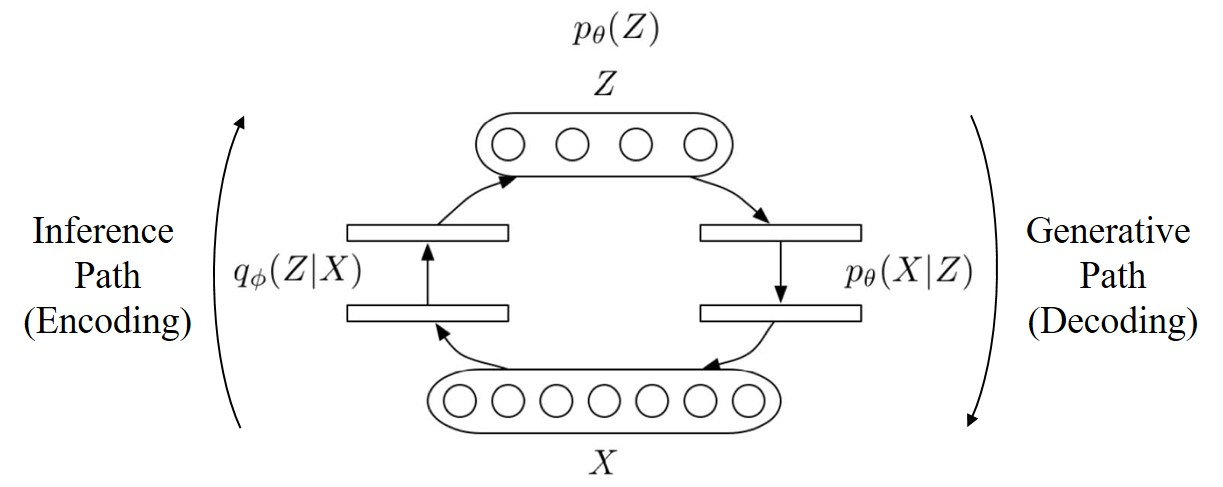
\includegraphics[width=12cm]{fig_8_2.jpg} 
	\caption{The diagram of VAE.}\label{fig_8_2}
\end{figure}
\subsection{ELBO: Generative Model Updates}
To maximize the ELBO w.r.t. $\theta$ (update the generative model), we need to be able to compute the gradients w.r.t. $\theta$. The idea is to apply a technique called \emph{stochastic approximation}. Specifically, with the observation that only the first term in ELBO depends on $\theta$ we can do the following
\begin{equation*}
\nabla_{\theta}\mathbb{E}_{q_{\phi}}[\log p_\theta({\bf x}|{\bf z})] = \mathbb{E}_{q_{\phi}}[\nabla_{\theta}\log p_\theta({\bf x}|{\bf z})].
\end{equation*}
Here we apply the Leibniz integral rule which allows us to exchange $\mathbb{E}_{q_\phi}$ and $\nabla_{\theta}$. This rule does not always hold but for all the cases we are interested in. For the expectation, if we have $q_\phi$ we can compute a simple Monte Carlo approximation of it by sampling from $q_\phi$. Therefore, we obtain
\begin{equation*}
\nabla_{\theta}\mathbb{E}_{q_{\phi}}[\log p_\theta({\bf x}|{\bf z})] \approx \frac{1}{L}\sum_{r=1}^{L} \nabla_{\theta}\log p_\theta({\bf x}|{\bf z}^{(r)}),\ {\bf z}^{(r)}\overset{i.i.d}{\sim}q_\phi(\cdot;{\bf x}),
\end{equation*}
where $L$ is the number of sample and is a hyperparameter. For a fixed ${\bf z}^{(r)}$, $\nabla_{\theta}\log p_\theta({\bf x}|{\bf z}^{(r)})$ is the network gradient which can be obtained with backpropagation. (As shown in Figure \ref{fig_8_2}, the generative model outputs a conditional probability distribution over ${\bf x}$ given ${\bf z}$ rather than a deterministic value. This is a little bit different from the networks we have seen.) This Monte Carlo approximation produces an unbiased gradient estimate (SGD). The gradient is obtained in a sense that is similar to supervised learning, where we have ${\bf z}$ as the input and use the output ${\bf x}$ to compute the gradient. To show how this is done, for a Gaussian observation model
\begin{equation}\label{eq_8_gau_obs}
p_\theta({\bf x}|{\bf z})=\mathcal{N}(F_\theta({\bf z}), {\bf I}),
\end{equation}
the gradient is generated via a squared error $\frac{1}{2}\|F_\theta({\bf z})-{\bf x}\|^2$.
\par The updates for the generative model turns out to be the easy part in the maximization of ELBO. The inference model performs approximate model inversion in a way that given ${\bf x}$ it finds a reasonable ${\bf z}$. Determine the gradient w.r.t. $\phi$ turns out to be more tricky, and we will discuss it in the next section.
\subsection{ELBO: Inference Model Updates}
Let us first look at the update step for the inference model in an abstract view. For a general function $\mathcal{L}({\bf x,z})$, given ${\bf x}$ and ${\bf z}\sim q_\phi({\bf z};{\bf x})$, the gradient w.r.t. $\phi$ of the expectation of $\mathcal{L}({\bf x,z})$ (w.r.t. $q_\phi$) is given by
\begin{equation*}
\nabla_\phi \mathbb{E}_{q_\phi}[\mathcal{L}({\bf x,z})] = \underbrace{\int \mathcal{L}({\bf x,z}) \nabla_\phi q_\phi({\bf z};{\bf x})d{\bf z}}_{\text{still intractable}}=\mathbb{E}[?]
\end{equation*}
where again we have applied the Leibniz rule. Different from the generative model, here the dependency on $\phi$ is in the expectation. We can apply the Leibniz rule, but the result is not obviously in an expectation form. Note that if so we can again apply the Monte Carlo approximation by sampling and averaging. Following this idea, one way to rewrite the gradient into a form of expectation is by applying the \emph{reinforce trick} (Williams 1992):
\begin{equation*}
\nabla_\phi \mathbb{E}_{q_\phi}[\mathcal{L}({\bf x,z})] =  \mathbb{E}_{q_\phi}[\mathcal{L}({\bf x,z})	\nabla_\phi\log q_\phi({\bf z};{\bf x})],
\end{equation*}
where we have used
\begin{equation*}
\nabla q = q\nabla\log q.
\end{equation*}
Then we can estimate the gradient via sampling, but despite the unbiasedness of this estimation, the variance is usually very high, which requires impractically large number of samples to guarantee a accurate estimation. Nevertheless, this reinforce trick can already be a feasible way to update the inference model. By doing so we have completed the map of optimizing VAEs.
\par Another way to make the gradient some expectations is by applying the \emph{re-parameterization trick}. Instead of allowing any variational distribution $q_\phi$, we use $q_\phi$ such that
\begin{equation*}
{\bf z} = g_\phi(\zeta;{\bf x})\quad \text{and}\quad{\bf z}\sim q_\phi({\bf z};{\bf x}).
\end{equation*}
where
\begin{equation*}
\zeta\sim \text{ simple distribution (e.g. }\mathcal{N}({\bf 0,I})).
\end{equation*}
What we are doing here is basically a change of variable. We transform a very simple random variable $\zeta$ using a function $g_\phi(\cdot;{\bf x})$ (${\bf x}$ is its parameter) such that the resulting random variable ${\bf z}=g_\phi(\zeta;{\bf x})$ obeys $q_\phi({\bf z};{\bf x})$, i.e. ${\bf z}\sim q_\phi({\bf z};{\bf x})$. With this re-parameterization, the gradient of expectation can be converted into expectation of gradient (known as \emph{stochastic backpropagation}). Specifically, first recall the law of the unconscious statistician (LOTUS) (\ref{eq_8_lotus}), we can rewrite the gradient of expectation as
\begin{align*}
\nabla_\phi \mathbb{E}_{{\bf z}\sim q_\phi}[\mathcal{L}({\bf x,z})] &= \nabla_\phi \mathbb{E}_{\zeta\sim\mathcal{N}({\bf 0,I})} [\mathcal{L}({\bf x},g_\phi(\zeta;{\bf x}))]\ ({\rm LOTUS})\\
&=\mathbb{E}_{\zeta}[\nabla_\phi \mathcal{L}({\bf x},g_\phi(\zeta;{\bf x}))]\ (\text{Leibniz rule})\\
&\approx \frac{1}{L}\sum_{r=1}^{L}[\nabla_\phi \mathcal{L}({\bf x},g_\phi(\zeta^{(r)};{\bf x}))],\ \zeta^{(r)}\overset{i.i.d.}{\sim}\mathcal{N}({\bf 0,I}),
\end{align*}
where $\zeta$ can obey other simple distributions as well. As an example, consider $\zeta\sim\mathcal{N}({\bf 0,I})$. If we define
\begin{equation*}
{\bf z} = g_\phi(\zeta;\underbrace{\mu,{\bf U}}_{\phi})=\mu +{\bf U}\zeta.
\end{equation*}
Then
\begin{equation*}
{\bf z}\sim \mathcal{N}(\mu,{\bf UU}^T).
\end{equation*}
In practice, it is often observed that re-parameterization trick leads to lower variance estimates than the reinforce trick, but this does not mean that the re-parameterization is in a sense consistently better than the other one (no theoretical results).
\subsection{Deep Latent Gaussian Models}
Now we look at an instantiation of the VAE framework we have just discussed about, namely the Deep Latent Gaussian Models (DLGM). In DLGM, we inject randomness in a simple form at each layer to the deep model.  Specifically, for each layer we define a noise variable
\begin{equation*}
{\bf z}^l\overset{i.i.d.}{\sim}\mathcal{N}({\bf 0,I}),\ l=1,\dots,L.
\end{equation*}
Let ${\bf x}^l$ be the activation for layer $l$. We start from the generative model of DLGM with top-down-indexed layers (we start from the $L$-th layer all the way to ${\bf x}^1$ from which we can sample data points). The forward propagate starts from the $L$-th layer with
\begin{equation*}
{\bf x}^L={\bf W}^L{\bf z}^L.
\end{equation*}
The intermediate hidden activities (latent random variables) act in the following way:
\begin{equation*}
{\bf x}^l=\underbrace{F^l({\bf x}^{l+1})}_{\rm deterministic}+\underbrace{{\bf W}^l{\bf z}^l}_{\rm stochastic},
\end{equation*}
where the first term is deterministic with the layer mapping $F^l$, and the index $l+1$ shows that we are propagating top-down; the second term shows that we always inject randomness in each layer (via a linear transform of a part of latent variable ${\bf z}=({\bf z}^1,\dots,{\bf z}^L)$, see also remark \ref{rmk_8_1}). The hidden layer (conditional) distribution is then
\begin{equation*}
{\bf x}^l|{\bf x}^{l+1}\sim \mathcal{N}\left(F^l({\bf x}^{l+1}),{{\bf W}^l{\bf W}^l}^T\right).
\end{equation*}
Finally, we generate pattern ${\bf x}\sim \pi({\bf x}^l)$, where $\pi(\cdot)$ is an observation/noise model with parameter ${\bf x}^1$ (as an example: the Gaussian observation model (\ref{eq_8_gau_obs})).

\par For the inference model of DLGM, first recall that given ${\bf x}$ the inference model helps to find ${\bf z}$ that we have to inject to the generative model to produce such a ${\bf x}$. In DLGM, ${\bf z}$ consist of all randomness injected in each layer (known as amortized inference):
\begin{equation*}
{\bf z} =({\bf z}^1,\dots,{\bf z}^L).
\end{equation*}
Assume we draw ${\bf z}^l$ independently. The variational distribution $q_\phi({\bf z};{\bf x})$ is given by
\begin{equation*}
q_\phi({\bf z};{\bf x})=\prod_{l=1}^{L}\mathcal{N}({\bf z}^l|\mu^l({\bf x}),{\bf C}^l({\bf x})),\quad {\bf C}^l({\bf x})={\bf U}^l({\bf x}){\bf U}^l({\bf x})^T,
\end{equation*}
where $\mu$ and $\bf U$ are represented by DNNs with input $\bf x$. The update equations for $\mu$ in the inference model can be obtained using the Bonnet formula (for ${\bf z}\sim \mathcal{N}(\mu,{\bf C})$):
\begin{equation*}
\nabla_\mu\mathbb{E}_{\bf z}[f({\bf z})]=\mathbb{E}_{\bf z}[\nabla_{\bf z} f({\bf z})].
\end{equation*}
Here's a brief proof for the Bonnet formula:
\begin{align*}
\nabla_{\mu_i}\mathbb{E}_{\mathcal{N}(\mu,{\bf C})}[f({\bf z})] &= \int  \nabla_{\mu_i} \mathcal{N}({\bf z}|\mu,{\bf C}) f({\bf z}) d{\bf z}\\
&=-\int \left[\nabla_{z_i}\mathcal{N}({\bf z}|\mu,{\bf C})\right] f({\bf z}) d{\bf z}\\
&=\left[\int\mathcal{N}({\bf z}|\mu,{\bf C}) f({\bf z}) d{\bf z}_{\neg i} \right]_{z_i=-\infty}^{z_i=\infty}+ \int \mathcal{N}({\bf z}|\mu,{\bf C}) \nabla_{z_i} f({\bf z}) d{\bf z}\\
&=\mathbb{E}_{\mathcal{N}(\mu,{\bf C})}[\nabla_{z_i}f({\bf z})].
\end{align*}
For ${\bf U}$, we can use the re-parameterization trick. Recall that we have ${\bf z}\sim \mathcal{N}(\mu,{\bf C})$, and this can be re-parameterized by ${\bf z}={\bf U}\zeta +\mu,\ \zeta\sim\mathcal{N}(0,{\bf I})$. Then LOTUS yields
\begin{equation*}
\nabla_{\bf U}\mathbb{E}_{\bf z}[f({\bf z})]=\nabla_{\bf U}\mathbb{E}_\zeta[f({\bf U}\zeta +\mu)]=\mathbb{E}_\zeta[\zeta{\bf g}^T],\ {\bf g}:=\nabla_\xi f(\xi)_{|\xi={\bf U}\zeta+\mu},
\end{equation*}
where we have used the chain rule for composition of a function with a linear function. Note that it should be $\mathbb{E}_\zeta[\zeta{\bf g}^T]$ rather than $\mathbb{E}_\zeta[\zeta^T{\bf g}]$ as in the slides.
\begin{remark}\label{rmk_8_1}
	In Figure \ref{fig_8_2}, the diagram seems to require the model (networks) to give $q_\phi({\bf z};{\bf x})$  at the last layer of the inference model. However, as the deep latent Gaussian models suggest, this is not the case in the sense that the model can generate the distribution of a part of ${\bf z}$ at the intermediate layers. So we see that the VAE shown in Figure \ref{fig_8_2} is an abstract framework, and $q_\phi({\bf z};{\bf x})$ and $p_\theta({\bf x}|{\bf z})$ don't even have to be produced by a deep model, but other models work as well.
\end{remark}
\begin{remark}
	In the original paper (Rezende et al. 2014), the Price's Theorem and Gaussian backpropagation refer to different things, so there might be some name misusing.
\end{remark}
Finally we can have a look at the big picture of DLGM. As illustrated in Figure \ref{fig_8_3}, DLGM consists of 2 parts: the generative model on the left and the recognition (inference) model on the right. The red arrows in the image represent propagation in learning, while the black ones are the forward passes. 
\par To generate new data point ${\bf x}$, we sample ${\bf z}^l\sim \mathcal{N}(\mu^l,{\bf C}^l)$ with given $(\mu^l,{\bf C}^l)$ (black horizontal dotted arrows); the activation ${\bf x}^l$ are sampled from $ \mathcal{N}\left(F^l({\bf x}^{l+1}),{{\bf W}^l{\bf W}^l}^T\right)$ (black vertical dotted arrows). The red arrows in generative model shows how the backpropagation goes along the layers. Given ${\bf x}_0$ and ${\bf z}$ produced by the inference model $q_\phi({\bf z}|{\bf x}_0)$, the gradients are obtained by the error $l(x_0,{\rm Gen}({\bf z}))$, where ${\rm Gen}({\bf z})$ is an output of the generative model with ${\bf z}$.
\par The inference model is similar. The forward pass represented by black arrows are deterministic given ${\bf x}$, since $\{\mu({\bf x}), {\bf C}({\bf x})\}$ are deterministic functions w.r.t. ${\bf x}$. The red dashed arrows are stochastic backpropagation, where we use the re-parameterization trick and need to sample $\zeta\sim \mathcal(0,{\bf I})$.
\begin{figure}[h] 
	\centering 
	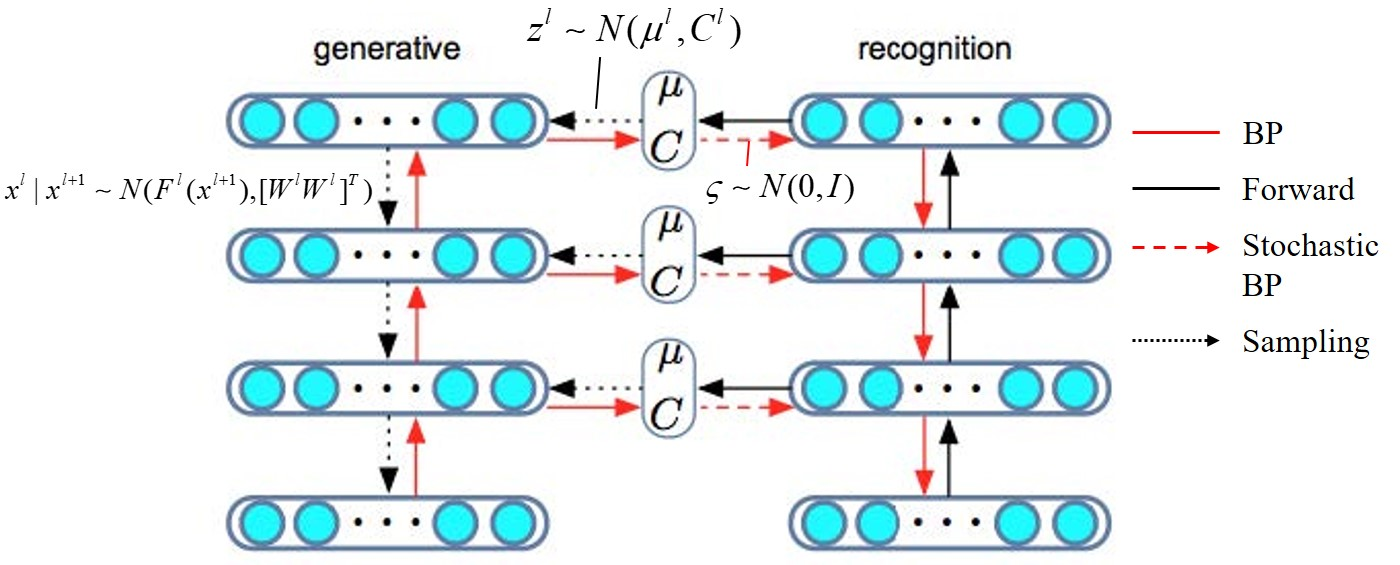
\includegraphics[width=12cm]{fig_8_3.jpg} 
	\caption{Learning and forward propagation scheme for Deep Latent Gaussian Models.}\label{fig_8_3}
\end{figure}
\par Here is some example generated by VAEs. As we can see that they are not bad but kind of blurry (Figure \ref{fig_8_4}). We will another type of model that is able to generate better results in the next section.
\begin{figure}[h] 
	\centering 
	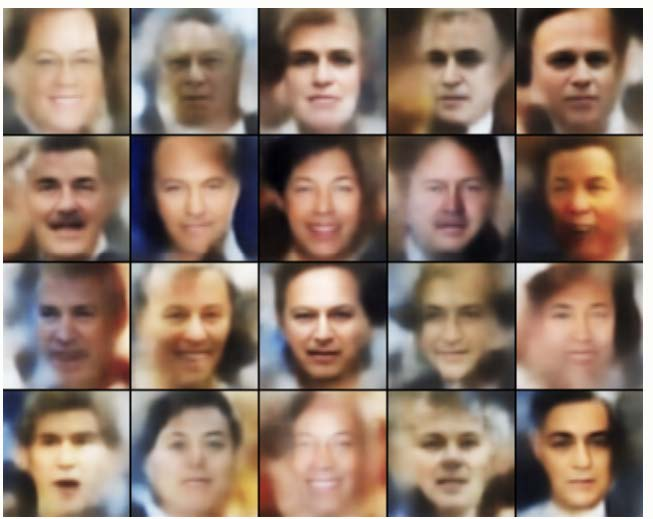
\includegraphics[width=6cm]{fig_8_4.jpg} 
	\caption{Face generation via VAEs.}\label{fig_8_4}
\end{figure}
\section{Generative Adversarial Networks}
GANs, proposed by Goodfellow et al.,2014, are something better known than VAEs. The idea is also more straightforward: given some data, say faces, generated by some devices and also some real faces, if there's a way that somehow we can discriminate these faces this could provide an error signal to the generator. In another word, we want to have a classifier/discriminator to train the generator.
\par Let us make this idea concrete by defining a formal classification problem, where we have a mixed source of data: half forms by the real ones and the other by the generated ones. Denote a data sample by ${\bf x}$ and the corresponding label by ${y}$ indicating whether it is real ($y=1$) or not ($y=0$), we can then define th joint distribution of $({\bf x},y)$ as mixture by
\begin{align*}
&\tilde{p}_\theta({\bf x},y=1)=P(y=1)P({\bf x}|y=1)=\frac{1}{2}p({\bf x})\\
&\tilde{p}_\theta({\bf x},y=0)=P(y=0)P({\bf x}|y=0)=\frac{1}{2}p_\theta({\bf x}),
\end{align*}
where $\tilde{p}_\theta$ denotes the distribution of mixed data with $p({\bf x})$ and $p_\theta({\bf x})$ representing the distribution of real data and generated data respectively. Before we discuss how this setting can benefit our learning, let us first think about what is the best can a discriminator do. The answer is given by the Bayes optimal classifier, i.e. making decision based on the posterior $P(y|{\bf x})$:
\begin{equation*}
P(y=1|{\bf x}) = q_\theta=\frac{p}{p+p_\theta},\ {\rm output}\ y=\begin{cases}
1 & {\rm if}\ q_\theta>\frac{1}{2}\\
0 & {\rm otherwise}
\end{cases}.
\end{equation*}
The goal of a generator is to generate samples that are indistinguishable from the real data, even for the best possible classifier, i.e. the Bayes optimal classifier. Specifically, we want to train a generator via minimizing the logistic likelihood for the discriminators, particularly for the best possible one:
\begin{equation*}
\theta\overset{\min}{\rightarrow}l^*(\theta):=\mathbb{E}_{\tilde{p}_\theta}[y\ln q_\theta({\bf x})+(1-y)\ln(1-q_\theta({\bf x}))].
\end{equation*}
It can be shown that
\begin{equation*}
l^*(\theta)={\rm JS}(p,p_\theta)-\ln 2,
\end{equation*}
where ${\rm JS}$ is the Jensen-Shannon divergence which measures distance between distributions. From this we can see that, to train a generator that minimize $l^*(\theta)$, we need to make $p_\theta \approx p$. In practice, we have no access to these two distributions and cannot compute the JS-divergence. The discussion here just aims at giving some theoretical intuition.
\par If we have no access to $p$ and $p_\theta$, the optimal classifier is in general inaccessible. Instead, we can define a classification model, just as in VAEs we introduce a second model, given by
\begin{equation*}
q_\phi:{\bf x}\rightarrow [0,1],\quad \phi\in\Phi,
\end{equation*}
where $\phi$ represent model parameters and $\Phi$ is the class of functions (weight space for DNN model). By optimality, plugging in any classifier to the logistic likelihood will result in a lower bound for $l^*(\theta)$, so to get it close to the Bayes optimal we take $\sup$ over $\Phi$:
\begin{equation*}
l^*(\theta)\geq\sup_{\phi\in\Phi}l(\theta,\phi),\quad l(\theta,\phi) :=\mathbb{E}_{\tilde{p}_\theta}[y\ln q_\phi({\bf x})+(1-y)\ln(1-q_\phi({\bf x}))].
\end{equation*}
Taking sup means finding the best classifier within the restricted family ${\Phi}$. While for the generator, it wants to make the likelihood low for all possible classifiers, which means that the training objective for the generator is defined implicitly over sup:
\begin{equation*}
\theta^*:=\mathop{\arg\min}_{\theta\in\Theta}\{\sup_{\phi\in\Phi}l(\theta,\phi)\},
\end{equation*}
where ${\Theta}$ is the class of functions for generative model from which the generator want to find a ${\theta}$ that minimize $\sup_{\phi\in\Phi}l(\theta,\phi)$. Note that in VAEs we maximize over both $\theta$ and $\phi$, but here we have an adversarial setting, also known as a \emph{saddle-point problem}. Despite we have already defined an optimization objective, explicitly performing inner sup is impractical, and solving saddle-point problem is in general very hard. Still there have been various methods from optimization and solving ``games''. But let's put these aside. The simplest thing one can do is a simultaneous SGD and Ascent (for the sup we need to do ascent instead of descent) by updating the parameters follow
\begin{align*}
&\theta^{t+1}=\theta^t-\eta \nabla_\theta l(\theta^t,\phi^t)\\
&\phi^{t+1}=\phi^t+\eta \nabla_\phi l(\theta^{t+1},\phi^t).
\end{align*}
Although this may diverge and has no theoretical guarantees as SGD for convex functions. Problematic cases that this fails can be easily constructed. However, this is just a staring point, and at least we can tell that one can easily train a classifier to distinguish VAE-generated data while the GANs can do better. Despite, the GANs are very hard to train, very expensive to train (many GPUs needed), and there is no clear evaluation metric (we don't know whether the models captures all important things), with efforts and proper tricks people have made it to use GANs to generate amazing results (Figure \ref{fig_8_1}).
\subsection{GANs v.s. VAEs}
GANs and VAEs are both generative models but have quite different characteristics. In this section we will compare the two generative models we have seen from several aspects:
\begin{itemize}
	\item Quality
	\begin{itemize}
		\item VAEs tend to generate blurry images. This is caused by pixel-wise factorization and local loss. (Recall the loss function for Gaussian observation models (\ref{eq_8_gau_obs}).) In this case, the high-frequency details are poorly correlated and hard to predict. 
		\item GANs generate sharper images. By training a discriminator, we get a ``perceptual'' loss.
	\end{itemize}
\begin{figure}[h] 
	\centering 
	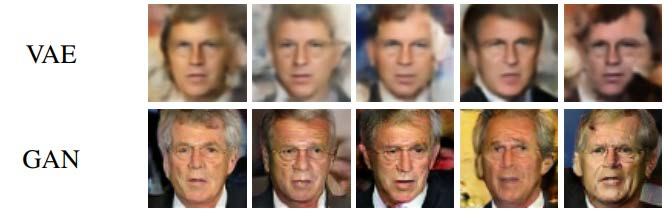
\includegraphics[width=6cm]{fig_8_GANs_VAEs.jpg} 
	\caption{Comparison of image quality.}\label{fig_8_GANs_VAEs}
\end{figure}
	\item Training
	\begin{itemize}
		\item GANs are very hard to train, where the architectures and hyperparameters play a crucial role. People have proposed many tricks and variants.
		\item VAEs are some what easier to train but not too easy (especially for other domains like text).
	\end{itemize}
	\item Applications
	\begin{itemize}
		\item GANs learn an implicit density and can only generate (samples).
		\item VAEs learn an explicit density with which we can sample and encode.
		\item Some approaches combine VAEs and GANs to take the best of both of worlds (VAE-GAN: VAE to gide the style of a GAN).
	\end{itemize}
\end{itemize}

\section{Autoregressive Models}
The last part of this chapter is about something less fascinating but easier and able to produce quite good results. These models have been used for many speech synthesis tasks.
\par Despite the generating power of VAEs and GANs, they requires complicated learning methods and are not always successful. Autoregressive models exploits a simpler strategy: generate output variable one at a time with the help of chain rule:
\begin{equation*}
p(x_1,\dots,x_m)=\prod_{t=1}^{m}p(x_t|x_{1:t-1}).
\end{equation*}
Take image synthesis for example, to generate image pixels, we can just give the pixels some order, and conditioning on what we already have to decide what to produce next. This is exactly the idea behind PixelCNN (A. van de Oord et al. 2016), where the network models a conditional distribution for every individual pixel given previous pixels (to the left and to the top in PixelCNN, but it is just a design choice).
\begin{figure}[h] 
	\centering 
	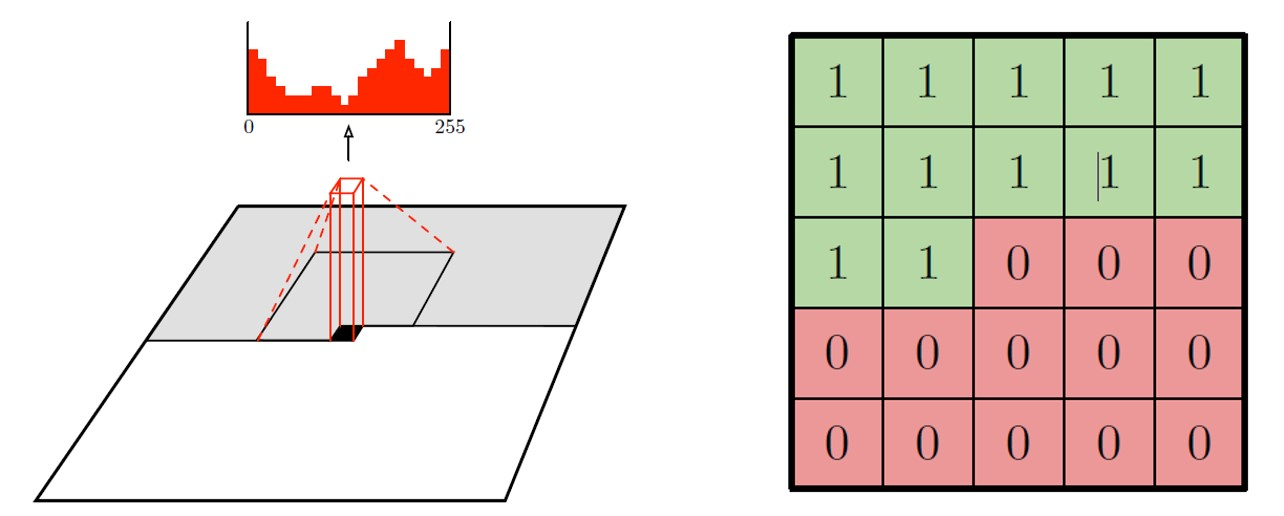
\includegraphics[width=10cm]{fig_8_5.jpg} 
	\caption{Left: PixelCNN uses previous generated pixels to help predict the next one. Right: the conditioning is equivalent to perform a masked convolution, this is why it is called CNN.}\label{fig_8_5}
\end{figure}
The way PixelCNN works is illustrated in Figure \ref{fig_8_5}. It model the joint distribution of pixels over image ${\bf x}$ as products of conditional distributions, where $x_i$ is a single pixel:
\begin{equation*}
p({\bf x})=\prod_{i=1}^{n^2}p(x_i|x_{1:i-1}),
\end{equation*}
where $x_{1:i-1}$ are the previously generated pixels. The ordering of pixels dependencies is in a raster scan order: row by row and pixel by pixel within every row. Also, PixelCNN doesn't condition on all previous pixels, but in a sense that only for local context (the left part of Figure \ref{fig_8_5}). This can be done with a masked convolution (apply a masked filter) as shown in the right of Figure \ref{fig_8_5}.
\par The prediction of PixelCNN is sequential: every time a pixel is predicted, and it is fed back into the network to predict the next pixel. One drawback is that this might be too slow. 
\begin{figure}[h] 
	\centering 
	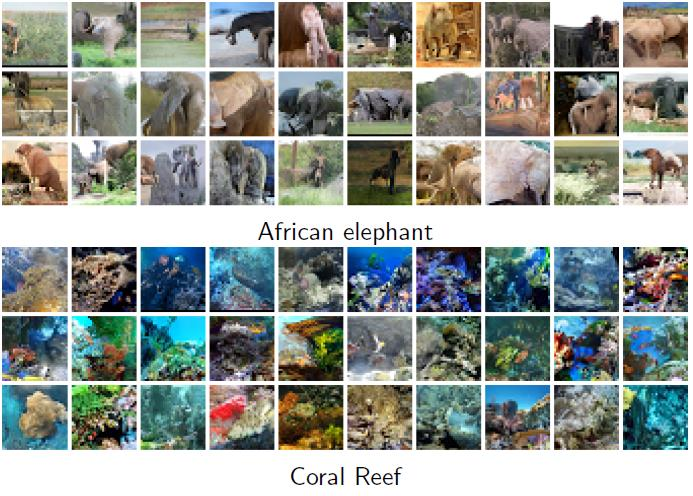
\includegraphics[width=10cm]{fig_8_6.jpg} 
	\caption{Some results from autoregressive model.}\label{fig_8_6}
\end{figure}
\par Figure \ref{fig_8_6} shows some example from PixelCNN. We see that although the quality of images are not as the ones produced by VAEs and GANs, PixelCNN still produces interesting results.
\end{document}